\documentclass[12pt]{article}

\RequirePackage{amsmath}
\RequirePackage{amsthm}
\RequirePackage{amssymb}
\RequirePackage[mathscr]{eucal}
\RequirePackage{mathtools}
\RequirePackage{etoolbox}
\usepackage[red]{zhoucx-notation}

\geometry{letterpaper, top = 1in, bottom = 1in, left = 1in, right = 1in}

% correct bad hyphenation here
\hyphenation{op-tical net-works semi-conduc-tor}

\pagestyle{fancy}
\fancyhf{}
\setlength{\headheight}{15pt}
\rhead{\textsf{Chapter 30, Graphical Models}}
\lhead{\textsf{Chenxi Zhou}}
\renewcommand{\headrulewidth}{1pt}
\cfoot{\thepage}


\newcommand{\titlebox}[4]{
\begin{tcolorbox}[colback = blue!5!white!95, colframe = blue!70!black
% colback = yellow!30!white, colframe = yellow!70!black 
]
  \noindent \textbf{ #1 } \hfill \textit{#2} 
  \begin{center}
  	 \LARGE{\textbf{#3}}
  \end{center}
\textbf{Chapter:} \textit{#4} \hfill \textbf{Prepared by:} \textit{Chenxi Zhou}
\end{tcolorbox}
}

\begin{document}

\titlebox{Notes on Statistical and Machine Learning}{}{Graphical Models}{30}
\thispagestyle{plain}

\vspace{10pt}

This note is prepared based on 
\begin{itemize}
	\item \textit{Chapter 8, Graphical Models} in \textcite{Bishop2016-tm}, and 
	\item \textit{Chapter 17, Undirected Graphical Models} in \textcite{Friedman2001-np}. 
\end{itemize}


\section*{I. Introduction} 

\begin{enumerate}[label=\textbf{\arabic*.}]

	\item \textbf{Why Graphical Models?:} \emph{Probabilistic graphical models}, or simply \emph{graphical models}, use diagrams to represent probability distributions. 
	
	They have the following advantages: 
	\begin{enumerate}
		\item They provide a simple way to visualize the structure of a probabilistic model and can be used to design and motivate new models; 
		\item Insights into the properties of the model, including conditional independence properties, can be obtained by inspection of the graph; 
		\item Complex computations, required to perform inference and learning in sophisticated models, can be expressed in terms of graphical manipulations, in which underlying mathematical expressions are carried along implicitly. 
	\end{enumerate}
	
	\item \textbf{Graph:} A \emph{graph}, denoted by $\calG$, consists of a pair $\parens{V, E}$, where $V$ is a set of vertices (node) and $E$ is a set of edges. In a probabilistic graphical model, 
	\begin{enumerate}
		\item each vertex represents a random variable (or group of random variables), and 
		\item the edges express probabilistic relationships between these variables. 
	\end{enumerate}
	
	\item \textbf{Directed Graphical Models:} In a \textit{directed graphical model}, also known as \textit{Bayesian networks}, the edges in the graph have a particular directionality indicated by arrows. 
	
	\textit{Remark.} Directed graphical models represent probability distributions that can be factored into products of conditional distributions, and have the potential for \textit{causal interpretations}. 
	
	\item \textbf{Undirected Graphical Models:} In an \textit{undirected graph}, also known as \emph{Markov random fields}, the edges have \emph{no} directional arrows. 
	
	\textit{Remark.} The absence of an edge between two vertices means that the corresponding random variables are conditionally independent, given the other variables.  
	
	\item \textbf{Challenges in Graphical Models:} The \textit{main challenges} in working with graphical models are 
	\begin{enumerate}
		\item model selection (choosing the structure of the graph), 
		\item estimation of the edge parameters from data, and 
		\item computation of marginal vertex probabilities and expectations from their joint distribution.
	\end{enumerate}
	
	\textit{Remark.} The last two tasks are called \emph{learning} and \emph{inference}, respectively, in the computer science literature. 
	
\end{enumerate}


\section*{II. Directed Graphical Model}

\subsection*{II.1 Introduction}

\begin{enumerate}[label=\textbf{\arabic*.}]

	\item \textbf{Motivating Example:} Consider the random variables $X$, $Y$ and $Z$ whose joint probability density function (pdf) is given by $f_{X,Y,Z}$. Using the product rule of probability, we have 
	\begin{align}
		f_{X,Y,Z} \parens{x, y, z} % = & \, f_{Z\vert X,Y} \parens{z \,\vert\, x, y} f_{XY} \parens{x, y} \nonumber \\ 
		= & \, f_{Z\vert X,Y} \parens{z \,\vert\, x, y} f_{Y \vert X} \parens{y \,\vert\, x} f_{X} \parens{x}, \label{eq-factor1}
	\end{align}
	where $f_{Z \vert X,Y}$ is the conditional pdf of $Z$ given $X = x$ and $Y = y$, $f_{Y \vert X}$ is the conditional pdf of $Y$ given $X = x$, and $f_X$ is the marginal pdf of $X$. 
	
	In order to create a diagram associated with the factorization \eqref{eq-factor1}, we do the following: 
	\begin{enumerate}
		\item Draw a vertex associated with each random variable; 
		\item For each conditional distribution, we add a directed edge (arrow) to the graph from the vertex corresponding to the variables on which the distribution is conditioned. 
	\end{enumerate}
	The resulting diagram is shown in Figure \ref{fig-factorization-1}. 
	\begin{figure}[h]
		\centering
		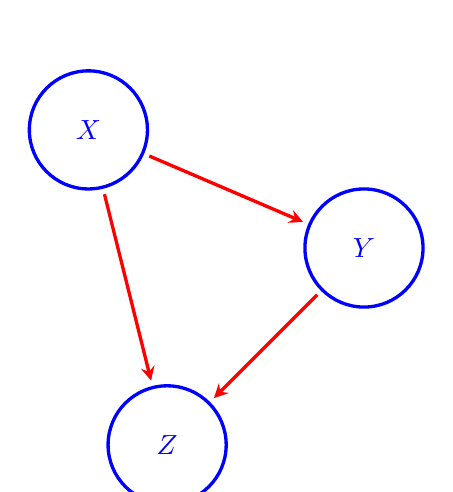
\begin{tikzpicture}
			\node[draw,circle,minimum size=1.5cm,minimum width=1.5cm,color=blue,very thick] (p1) at (0,0){$X$};
			\node[draw,circle,minimum size=1.5cm,minimum width=1.5cm,color=blue,very thick] (p2) at (3.5,-1.5){$Y$};
			\node[draw,circle,minimum size=1.5cm,minimum width=1.5cm,color=blue,very thick] (p3) at (1,-4){$Z$}; 
			\draw (p1) edge [->,>=stealth,shorten <=2pt, shorten >=2pt, very thick, color = red] (p3); 
			\draw (p2) edge [->,>=stealth,shorten <=2pt, shorten >=2pt, very thick, color = red] (p3); 
			\draw (p1) edge [->,>=stealth,shorten <=2pt, shorten >=2pt, very thick, color = red] (p2); 
		\end{tikzpicture}
		\captionsetup{width=.7\linewidth}
		\caption{Diagram associated with the factorization \eqref{eq-factor1}.}
		\label{fig-factorization-1}
	\end{figure}
	
	\item \textbf{Parent and Child Vertices:} If there is a directed edge going from a vertex $A$ to a vertex $B$, then we say that 
	\begin{enumerate}
		\item the vertex $A$ is the \emph{parent} of the vertex $B$, and 
		\item the vertex $B$ is the \emph{child} of vertex $A$. 
	\end{enumerate}
	
%	\item \textbf{Extensions to $M$ Random Variables:} Suppose we have $M$ random variables whose joint pdf is given by $f_{X_1,X_2,\cdots,X_M}$. We can express $f_{X_1,X_2,\cdots,X_M}$ as 
%	\begin{align*}
%		f_{X_1, X_2, \cdots, X_M} \parens{x_1, x_2, \cdots, x_M} = \bracks[\Bigg]{\prod_{m=1}^M f_{X_m \vert X_1, \cdots, X_{m-1}} \parens{x_m \,\vert\, x_1, \cdots, x_{m-1}}} \times f_{X_1} \parens{x_1}, 
%	\end{align*}
%	where $f_{X_m \vert X_1, \cdots, X_{m-1}}$ is the conditional pdf of $X_m$ on $X_1 = x_1$, $\cdots$, $X_{m-1} = x_{m-1}$, and $f_{X_1}$ is the marginal pdf of $X_1$. 
	
	\item \textbf{Fully Connected Graph:} A graph is said to be \emph{full connected} if there is a link between every pair of vertices. 
	
	\item \textbf{Relationship between a Given Directed Graph and Distribution of Random Variables:} 
	\begin{enumerate}
		\item The joint distribution defined by a graph is given by the product, over all of the nodes of the graph, of a conditional distribution for each node conditioned on the variables corresponding to the \emph{parents} of that node in the graph. Mathematically, for a graph with $m$ nodes, the joint distribution can be factored as 
		\begin{align}\label{eq-factorization-2}
			f_{X_1, X_2, \cdots, X_m} \parens{x_1, x_2, \cdots, x_m} = \prod_{j=1}^m f_{X_j \vert \mathrm{pa}_j} \parens{x_j \,\vert\, \mathrm{pa}_j}, 
		\end{align}
		where $\mathrm{pa}_j$ denotes the set of \emph{parents} of $x_j$. 
		
		\textit{Remark.} Equation \eqref{eq-factorization-2} expresses the \emph{factorization properties} of the joint distribution for a directed graphical model. 
		
		\item Conversely, given the factorization in the form of \eqref{eq-factorization-2}, we can associate sets of variables with the nodes of a directed graph. 
	
	\end{enumerate}
	
	\item \textbf{Directed Acyclic Graphs:} A graph is said to be a \textit{directed acyclic graph} if it contains no directed cycles, i.e., there are \emph{no} closed paths within the graph such that we can move from node to node along links following the direction of the arrows and end up back at the starting node. 
	
	\textit{Remark.} A directed acyclic graph is equivalent to that there exists an ordering of the nodes such that there are \emph{no} links that go from any node to any lower numbered node. 
	
	\item \textbf{Practical Applications of Directed Acyclic Graphs:} Typically, 
	\begin{enumerate}
		\item the higher-numbered variables correspond to terminal nodes of the graph that represent the \emph{observations}, 
		\item the lower-numbered variables correspond to latent variables. 
	\end{enumerate}
	The primary role of the latent variables is to allow a complicated distribution over the observed variables to be represented in terms of a model constructed from simpler conditional distributions. 

	\item \textbf{Ancestral Sampling:} 
	\begin{enumerate}
		
		\item \textit{Setup:} Consider a joint pdf over $m$ random variables factorized according to \eqref{eq-factorization-2} corresponding to a directed acyclic graph. Suppose the $m$ variables have been ordered such that there are no links from any node to any lower numbered node. 
		
		\item \textit{Goal:} Our goal is to draw a sample $X_1, X_2, \cdots, X_m$ from the joint distribution. 
		
		\item \textit{Procedure:} 
		\begin{enumerate}
			\item Start from the lowest-numbered node and draw a sample from the distribution $f_{X_1}$, which we call $X_1$; 
			\item Work through each of the nodes in order, so that for node $j$, we draw a sample from the conditional distribution $f_{X_j \vert \mathrm{pa}_j}$ in which the parent variables have been set to their sampled values. 
			\item Continue the preceding step until $j = m$. 
		\end{enumerate}
		
		\item \textit{Remarks:} 
		\begin{enumerate}
			\item Note that, at each stage, the parent values will \emph{always} be available because they correspond to lower-numbered nodes that have already been sampled. 
			\item To obtain a sample from some \emph{marginal} distribution corresponding to a subset of the random variables, we simply take the sampled values for the required nodes and \emph{ignore} the sampled values for the remaining nodes. 
		\end{enumerate}
		
	\end{enumerate}

\end{enumerate}

\subsection*{II.2 Discrete Random Variables}

\begin{enumerate}[label=\textbf{\arabic*.}]

	\item \textbf{Setup:} We assume all nodes correspond to discrete random variables. 
	
	\item \textbf{Univariate Discrete Random Variable:} We consider a single random variable that can take on $K$ distinct values. The corresponding pmf can be written as 
	\begin{align*}
		\Pr \parens{X = \bx} = \prod_{k=1}^K \mu_{k}^{x_k}, 
	\end{align*}
	which is governed by the parameter $\bmu := \parens{\mu_1, \mu_2, \cdots, \mu_K}^\top \in \Real^K$ with $\sum_{k=1}^K \mu_k = 1$. In addition, $\bx := \parens{x_1, x_2, \cdots, x_K}^\top \in \Real^K$ and exactly one component is equal to 1 and all others are 0. 
	
	\textit{Number of parameters to be determined:} Due to the unity constraint, only $K-1$ values for $\mu_k$ need to be specified in order to define the distribution. 
	
	\item \textbf{Bivariate Discrete Random Variable:} Suppose we have two discrete random variables $X_1$ and $X_2$, each of which can take on $K$ different values. 
	
	Let the probability of observing exactly the $k$-th component in $X_1$ equal to 1 and exactly the $\ell$-th component in $X_2$ equal to 1 be $\mu_{k,\ell}$. The joint pmf of $X_1$ and $X_2$ is 
	\begin{align*}
		\Pr \parens{X_1 = \bx_1, X_2 = \bx_2} = \prod_{k=1}^K \prod_{\ell=1}^K \mu_{k,\ell}^{x_{1,k} x_{2,\ell}}, 
	\end{align*}
	where $\bx_1 = \parens{x_{1,1}, x_{1,2}, \cdots, x_{1,K}}^\top \in \Real^K$ and $\bx_2 = \parens{x_{2,1}, x_{2,2}, \cdots, x_{2,K}}^\top \in \Real^K$. 
	
	\textit{Number of parameters to be determined:} Since the parameters $\sets{\mu_{k,\ell}}_{k,\ell}$ must satisfy $\sum_{k=1}^K \sum_{\ell=1}^K \mu_{k,\ell} = 1$, the distribution is governed by $K^2-1$ parameters in total. 
	
	\item \textbf{Bivariate Discrete Random Variable --- Case 1:} We can rewrite the joint pmf of $X_1$ and $X_2$ as 
	\begin{align*}
		\Pr \parens{X_1 = \bx_1, X_2 = \bx_2} = \Pr \parens{X_2 = \bx_2 \,\vert\, X_1 = \bx_1} \Pr \parens{X_1 = \bx_1}, 
	\end{align*}
	corresponding to a two-node graph with a link going from the $X_1$ node to the $X_2$ node (see Figure \ref{fig-factorization-2}). 
	
	\begin{figure}[h]
		\centering
		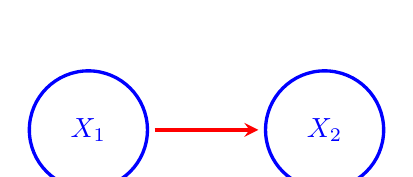
\begin{tikzpicture}
			\node[draw,circle,minimum size=1.5cm,minimum width=1.5cm,color=blue,very thick] (p1) at (0,0){$X_1$};
			\node[draw,circle,minimum size=1.5cm,minimum width=1.5cm,color=blue,very thick] (p2) at (3,0){$X_2$};
			\draw (p1) edge [->,>=stealth,shorten <=2pt, shorten >=2pt, very thick, color = red] (p2); 
		\end{tikzpicture}
		\captionsetup{width=.7\linewidth}
		\caption{Diagram associated with bivariate random variable case where $X_2$ is conditional on $X_1$.}
		\label{fig-factorization-2}
	\end{figure}
	
	The marginal distribution $f_{X_1}$ is governed by $K - 1$ parameters. The conditional distribution $f_{X_2 \vert X_1}$ requires the specification of $K - 1$ parameters for \emph{each} of the $K$ possible values of $X_1$. The total number of parameters that must be specified in the joint distribution is then 
	\begin{align*}
		\parens{K - 1} + K \times \parens{K - 1} = K^2 - 1. 
	\end{align*}
	
	\item \textbf{Bivariate Discrete Random Variable --- Case 2:} We assume the random variables $X_1$ and $X_2$ are independent, corresponding to the graphical model shown in \eqref{fig-factorization-3}. 
	
	\begin{figure}[h]
		\centering
		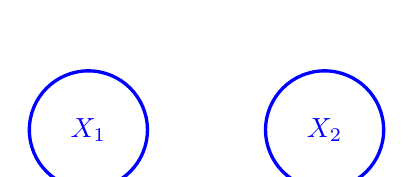
\begin{tikzpicture}
			\node[draw,circle,minimum size=1.5cm,minimum width=1.5cm,color=blue,very thick] (p1) at (0,0){$X_1$};
			\node[draw,circle,minimum size=1.5cm,minimum width=1.5cm,color=blue,very thick] (p2) at (3,0){$X_2$};
		\end{tikzpicture}
		\captionsetup{width=.7\linewidth}
		\caption{Diagram associated with bivariate random variable case where $X_1$ and $X_2$ are independent.}
		\label{fig-factorization-3}
	\end{figure}
	
	Then, the total number of parameters is $2 \times \parens{K-1}$. 
	
	\item \textbf{$m$-variate Discrete Random Variable:} We further extent to the case of $m$ discrete random variables, and assume each of $m$ random variables can take on $K$ distinct values. 
	\begin{enumerate}
		\item If we do \emph{not} put any constraints on the distribution and the corresponding directed acyclic graph is fully connected, the total number of parameters we need to determine to specify the distribution is $K^m-1$. 
		\item If we assume that $X_1, X_2, \cdots, X_m$ are all independent, the total number of parameters we need to determine to specify the distribution is $m \parens{K-1}$. 
		\item We can also make some assumptions on the independence among $X_1, X_2, \cdots, X_m$ so that the resulting graph is between full connectivity and full independence. As one example, assume the joint pmf of $X_1, X_2, \cdots, X_m$ can be factorized as 
		\begin{align*}
			& \, \Pr \parens{X_1 = \bx_1, X_2 = \bx_2, \cdots, X_m = \bx_m} \\ 
			& \qquad \qquad \qquad \qquad = \Pr \parens{X_1 = \bx_1} \prod_{j=2}^m \Pr \parens{X_j = \bx_j \,\vert\, X_{j-1} = \bx_{j-1}}. 
		\end{align*}
		The corresponding graph is given by Figure \ref{fig-factorization-4}. 
		\begin{figure}[t]
		\centering
		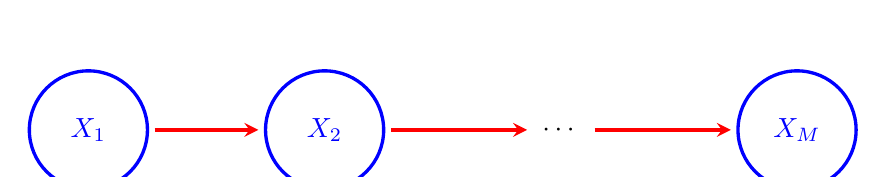
\begin{tikzpicture}
			\node[draw,circle,minimum size=1.5cm,minimum width=1.5cm,color=blue,very thick] (p1) at (0,0){$X_1$};
			\node[draw,circle,minimum size=1.5cm,minimum width=1.5cm,color=blue,very thick] (p2) at (3,0){$X_2$};
			\node (p3) at (6,0){$\cdots$}; 
			\node[draw,circle,minimum size=1.5cm,minimum width=1.5cm,color=blue,very thick] (p4) at (9,0){$X_M$};
			\draw (p1) edge [->,>=stealth,shorten <=2pt, shorten >=2pt, very thick, color = red] (p2); 
			\draw (p2) edge [->,>=stealth,shorten <=2pt, shorten >=2pt, very thick, color = red] (p3); 
			\draw (p3) edge [->,>=stealth,shorten <=2pt, shorten >=2pt, very thick, color = red] (p4); 
		\end{tikzpicture}
		\captionsetup{width=.7\linewidth}
		\caption{A special case of $M$-variate discrete random variable.}
		\label{fig-factorization-4}
	\end{figure}
	In this case, 
	\begin{enumerate}
		\item the total number of parameters to determine the distribution of $X_1$ is $K-1$, 
		\item the total number of parameters to determine the distribution of $X_j$ given $X_{j-1}$ is $K \parens{K-1}$, 
	\end{enumerate}
	so that the total number of parameters to determine the distribution of $X_1, X_2, \cdots, X_m$ is 
	\begin{align*}
		\parens{K - 1} + \parens{m - 1} K \parens{K-1} = m K^2 + , 
	\end{align*}
	which grows \emph{quadratically} in $K$ and grows \emph{linearly} (rather than exponentially) with the length $m$ of the chain. 
	\end{enumerate}
	
	\item \textbf{Parameter Sharing:} Another way of reducing the number of independent parameters is through \emph{parameter sharing}. 
	
	For example, one can assume that, in Figure \ref{fig-factorization-4}, all of the conditional distributions 
	\begin{align*}
		\Pr \parens{X_{j} = \bx_j \,\vert\, X_{j-1} = \bx_{j-1}}, \qquad \text{ for all } j = 2, \cdots, m, 
	\end{align*}
	are governed by the \emph{same} set of $K \parens{K-1}$ parameters. Together with the $K-1$ parameters governing the distribution of $X_1$, this gives a total of 
	\begin{align*}
		\parens{K-1} + K \parens{K-1} = K^2-1
	\end{align*}
	parameters that need to be specified in order to define the joint distribution. 

\end{enumerate}


\subsection*{II.3 Linear Gaussian Models}

\begin{enumerate}[label=\textbf{\arabic*.}]

	\item \textbf{Setup and Assumptions:} Consider an arbitrary directed acyclic graph over $m$ variables in which the $j$-th node represents a single continuous random variable $X_j$ having a Gaussian distribution with 
	\begin{enumerate}
		\item the mean being a linear combination of the states of its \emph{parent} nodes $\mathrm{pa}_j$ of the $j$-th node, and 
		\item the variance being $\sigma_j^2$, 
	\end{enumerate}
	that is, 
	\begin{align}\label{eq-linear-gau-1}
		X_j \,\vert\, \mathrm{pa}_j \sim \Normal \parens[\Bigg]{b_j + \sum_{\sets{\ell \vert X_\ell \in \mathrm{pa}_j}} w_{j, \ell} X_{\ell}, \sigma_j^2}. 
	\end{align}
	% In \eqref{eq-linear-gau-1}, $w_{j, \ell}$ and $b_j$ are parameters governing the mean, and $\sigma_j^2$ is the variance of the conditional distribution for $X_j$. 
	
	\item \textbf{Joint Density Function:} The logarithm of the joint density function of all nodes is 
	\begin{align}
		& \sum_{j=1}^m \log \varphi \parens[\Bigg]{X_j \,\Bigg\vert\, b_j + \sum_{\sets{\ell \vert X_\ell \in \mathrm{pa}_j}} w_{j, \ell} X_{\ell}, \sigma_j^2} \nonumber \\ 
		& \qquad \qquad = - \frac{1}{2} \sum_{j=1}^m \frac{1}{\sigma_j^2} \parens[\Bigg]{X_j - b_j - \sum_{\sets{\ell \vert X_\ell \in \mathrm{pa}_j}} w_{j, \ell} X_{\ell}}^2 - \frac{1}{2} \sum_{j=1}^m \log \sigma_j^2 + \text{const}, 
	\end{align}
	where ``const'' denotes terms that are independent of $\sets{b_j}_{j}$, $\sets{w_{j, \ell}}_{j, \ell}$ and $\sets{\sigma_j^2}_j$ and $X_1, X_2, \cdots, X_m$. 
	
	In particular, note that the joint density function of all nodes is a Gaussian density function, i.e., $\parens{X_1, X_2, \cdots, X_m}$ has a multivariate Gaussian distribution. 
	
	\item \textbf{Determining Mean and Variance of $\parens{X_1, X_2, \cdots, X_m}$:} Assume that the nodes are numbered such that each node has a higher number than its parents. We can determine the mean and covariance of the joint distribution \emph{recursively}. 
	
	For all $j = 1, 2, \cdots, m$, we can rewrite \eqref{eq-linear-gau-1} as 
	\begin{align}\label{eq-linear-gau-2}
		X_j \,\vert\, \mathrm{pa}_j = b_j + \sum_{\sets{\ell \vert X_\ell \in \mathrm{pa}_j}} w_{j, \ell} X_{\ell} + \sigma_j \varepsilon_j, 
	\end{align}
	where $\parens{\varepsilon_1, \varepsilon_2, \cdots, \varepsilon_m}^\top \sim \Normal_m \parens{\boldzero_m, \bI_m}$. 
	\begin{enumerate}
		\item \textit{Determining the Mean:} Taking the expectation of \eqref{eq-linear-gau-2} yields 
		\begin{align*}
			\E \bracks{X_j} = & \, \E \bracks[\big]{\E \bracks{X_j \,\vert\, \mathrm{pa}_j}} \\ 
			= & \, \E \bracks[\bigg]{b_j + \sum_{\sets{\ell \vert X_\ell \in \mathrm{pa}_j}} w_{j, \ell} X_{\ell} + \sigma_j \varepsilon_j} \\ 
			= & \, b_j + \sum_{\sets{\ell \vert X_\ell \in \mathrm{pa}_j}} w_{j, \ell} X_{\ell}. 
		\end{align*}
		Thus, we can determine $\parens{\E \bracks{X_1}, \E \bracks{X_2}, \cdots, \E \bracks{X_m}}^\top$ by starting at the lowest numbered node and working recursively through the graph. 
		
		\item \textit{Determining the Covariance:} The covariance between $X_j$ and $X_k$, for all $j, k = 1, 2, \cdots, m$, is 
		\begin{align*}
			\cov \parens{X_j, X_k} = & \, \E \bracks[\Big]{\parens{X_j - \E \bracks{X_j}} \parens{X_k - \E \bracks{X_k}}} \\ 
			% = & \, \E \bracks[\Bigg]{\parens{X_j - \E \bracks{X_j}} \parens[\Bigg]{\sum_{\sets{\ell \vert \ell \in \mathrm{pa}_k}} w_{k, \ell} \parens{X_{\ell} - \E \bracks{X_{\ell}} } + \sigma_k \varepsilon_k} } \\ 
			= & \, \sum_{\sets{\ell \vert \ell \in \mathrm{pa}_j}} \sum_{\sets{\ell' \vert \ell' \in \mathrm{pa}_k}} w_{j, \ell} w_{k, \ell'} \cov \parens{X_{\ell}, X_{\ell'}} + \sigma_k^2 \indic_{\sets{j = k}}, 
		\end{align*}
		where 
		\begin{align*}
			\indic_{\sets{j = k}} = \begin{cases}
				1, & \, \text{ if } j = k, \\ 
				0, & \, \text{ otherwise}. 
			\end{cases}
		\end{align*}
		It follows that the covariance can similarly be evaluated recursively starting from the lowest numbered node. 
	\end{enumerate}
	
	\item \textbf{Special Case 1:} Suppose that there are \emph{no} links in the graph so that all random variables are independent. 
	\begin{enumerate}
		\item \textit{Reduction of Number of Parameters:} There are no parameters $w_{j, \ell}$'s. One only needs to determine $m$ parameters $b_1, b_2, \cdots, b_m$ for the mean and $m$ parameters $\sigma_1^2, \sigma_2^2, \cdots, \sigma_m^2$ for the variance. 
		\item \textit{Mean Parameters:} The mean $\parens{\E \bracks{X_1}, \E \bracks{X_2}, \cdots, \E \bracks{X_m}}^\top$ is given by  
		\begin{align*}
			\parens{b_1, b_2, \cdots, b_m}^\top. 
		\end{align*}
		\item \textit{Covariance Matrix:} The covariance matrix is diagonal of the form 
		\begin{align*}
			\diag \parens{\sigma_1^2, \sigma_2^2, \cdots, \sigma_m^2}. 
		\end{align*}
	\end{enumerate}
	
	\item \textbf{Special Case 2:} Consider a fully connected graph in which each node has all lower numbered nodes as parents. 
	\begin{enumerate}
		\item \textit{Total Number of Weight Parameters:} The matrix $w_{j, \ell}$ has $j - 1$ entries on the $j$-th row and hence is a lower triangular matrix, giving a total of $m \parens{m - 1}/2$ parameters to determine. 
		\item \textit{Total Number of Parameters in the Mean:} The parameters in the mean to be determined are $\sets{w_{j, \ell}}_{j, \ell}$ and $\sets{b_j}_j$, giving a total of $m \parens{m + 1}/2$ parameters to determine. 
		\item \textit{Total Number of Parameters in the Covariance Matrix:} The parameters in the covariance matrix to be determined are $\sets{w_{j, \ell}}_{j, \ell}$ and $\sets{\sigma_j^2}_j$, giving a total of $M \parens{M + 1}/2$ parameters to determine. 
		\item \textit{Summary:} In this special case, the total number of parameters to be determined is 
		\begin{align*}
			\frac{m \parens{m-1}}{2} + m + m = \frac{m \parens{m + 3}}{2}. 
		\end{align*}
	\end{enumerate}
	
	\item \textbf{Special case 3:} Consider the intermediate level of complexity of three random variables shown in Figure \ref{fig-factorization-5}. 
	
	\begin{figure}[h]
		\centering
		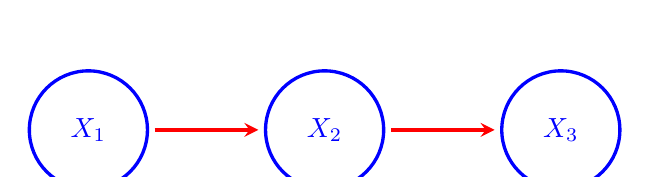
\begin{tikzpicture}
			\node[draw,circle,minimum size=1.5cm,minimum width=1.5cm,color=blue,very thick] (p1) at (0,0){$X_1$};
			\node[draw,circle,minimum size=1.5cm,minimum width=1.5cm,color=blue,very thick] (p2) at (3,0){$X_2$};
			\node[draw,circle,minimum size=1.5cm,minimum width=1.5cm,color=blue,very thick] (p3) at (6,0){$X_3$};
			\draw (p1) edge [->,>=stealth,shorten <=2pt, shorten >=2pt, very thick, color = red] (p2); 
			\draw (p2) edge [->,>=stealth,shorten <=2pt, shorten >=2pt, very thick, color = red] (p3); 
		\end{tikzpicture}
		\captionsetup{width=.7\linewidth}
		\caption{A special case of trivariate discrete random variable.}
		\label{fig-factorization-5}
	\end{figure}
	
	By inspecting the structure of the graph and using the results above, the mean vector is given by 
	\begin{align*}
		\begin{pmatrix}
			\E \bracks{X_1} \\ \E \bracks{X_2} \\ \E \bracks{X_3}
		\end{pmatrix} = \begin{pmatrix}
			b_1 \\ 
			b_2 + w_{2,1} X_1 \\ 
			b_3 + w_{3,2} X_2 + w_{3,2} w_{2,1} X_1
		\end{pmatrix}, 
	\end{align*}
	and the covariance matrix is given by 
	\begin{align*}
		\begin{pmatrix}
			\sigma_1^2 & w_{2,1} \sigma_1^2 & w_{3,2} w_{2,1} \sigma_1^2 \\ 
			w_{2,1} \sigma_1^2 & \sigma_2^2 + w_{2,1}^2 \sigma_1^2 & w_{3,2} \parens{\sigma_2^2 + w_{2,1}^2 \sigma_1^2} \\ 
			w_{3,2} w_{2,1} \sigma_1^2 & w_{3,2} \parens{\sigma_2^2 + w_{2,1}^2 \sigma_1^2} & \sigma_3^2 + w_{3,2} \parens{\sigma_2^2 + w_{2,1}^2 \sigma_1^2}
		\end{pmatrix}. 
	\end{align*}
\end{enumerate}


\section*{III. Conditional Independence}

\begin{enumerate}[label=\textbf{\arabic*.}]

	\item \textbf{Conditional Independence:} Consider three random variables $X$, $Y$ and $Z$, and suppose that the conditional distribution of $X$, given $Y$ and $Z$, does \emph{not} depend on $Y$, that is, 
	\begin{align}
		f_{X \vert Y, Z} \parens{x \,\vert\, y, z} = f_{X \vert Z} \parens{x \,\vert\, z}. 
	\end{align}
	We say that $X$ is \emph{conditionally independent} of $Y$ given $Z$, and is denote by 
	\begin{align}
		X \indep Y \,\vert\, Z. 
	\end{align}
	
	\textit{Remark.} Alternatively, assuming $X$ is conditionally independent of $Y$ given $Z$, we have 
	\begin{align*}
		f_{X, Y \vert Z} \parens{x, y \,\vert\, z} = & \, f_{X \vert Y, Z} \parens{x \,\vert\, y, z} f_{Y \vert Z} \parens{y \,\vert\, z} \\ 
		= & \, f_{X \vert Z} \parens{x \,\vert\, z} f_{Y \vert Z} \parens{y \,\vert\, z}. 
	\end{align*}
	Thus, conditioning on $Z$, the joint distribution of $X$ and $Y$ factorizes into the product of the marginal distribution of $X$ and that of $Y$ (again both conditioned on $Z$ \emph{only}). This says that the variables $X$ and $Y$ are statistically independent, given $Z$. 
	
	\item \textbf{Connection between Conditional Independence and Graphical Models:} An important and elegant feature of graphical models is that conditional independence properties of the joint distribution can be read directly from the graph \emph{without} having to perform any analytical manipulations. 
	
	\item \textbf{Example 1:} Consider the example shown in Figure \ref{fig-conditional-indep-1}. 
	
	\begin{figure}[h]
		\centering
		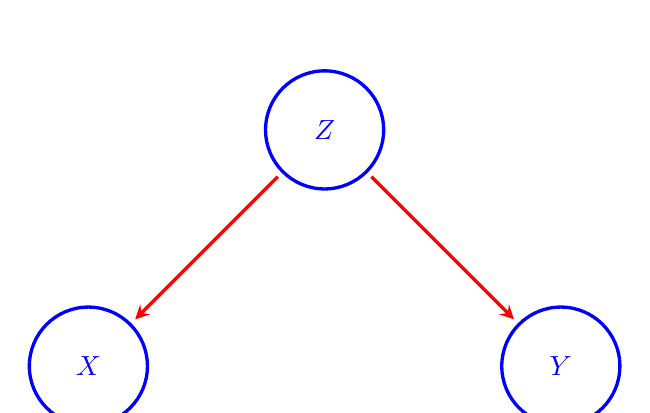
\begin{tikzpicture}
			\node[draw,circle,minimum size=1.5cm,minimum width=1.5cm,color=blue,very thick] (p1) at (3,0){$Z$};
			\node[draw,circle,minimum size=1.5cm,minimum width=1.5cm,color=blue,very thick] (p2) at (0,-3){$X$};
			\node[draw,circle,minimum size=1.5cm,minimum width=1.5cm,color=blue,very thick] (p3) at (6,-3){$Y$};
			\draw (p1) edge [->,>=stealth,shorten <=2pt, shorten >=2pt, very thick, color = red] (p2); 
			\draw (p1) edge [->,>=stealth,shorten <=2pt, shorten >=2pt, very thick, color = red] (p3); 
		\end{tikzpicture}
		\captionsetup{width=.7\linewidth}
		\caption{Example 1 of conditional independence.}
		\label{fig-conditional-indep-1}
	\end{figure}
	
	The corresponding joint pdf can be factorized as 
	\begin{align*}
		f_{X, Y, Z} \parens{x, y, z} = f_{X \vert Z} \parens{x \,\vert\, z} f_{Y \vert Z} \parens{y \,\vert\, z} f_{Z} \parens{z}. 
	\end{align*}
	Marginalizing with respect to $Z$ yields 
	\begin{align*}
		f_{X, Y} \parens{x, y} = \int f_{X, Y, Z} \parens{x, y, z} \diff z = \int f_{X \vert Z} \parens{x \,\vert\, z} f_{Y \vert Z} \parens{y \,\vert\, z} f_{Z} \parens{z} \diff z. 
	\end{align*}
	In general, we cannot factorize the preceding equation into $f_X \parens{x} f_Y \parens{y}$ and so $X$ and $Y$ are \emph{not} independent. 
	
	Now, conditioning on $Z$, we have 
	\begin{align*}
		f_{X, Y \vert Z} = \frac{f_{X, Y, Z} \parens{x, y, z}}{f_{Z} \parens{z}} = f_{X \vert Z} \parens{x \,\vert\, z} f_{Y \vert Z} \parens{y \,\vert\, z}, 
	\end{align*}
	and we obtain $X \indep Y \,\vert\, Z$. 
	
	\textit{Remark.} The node $Z$ is said to be \emph{tail-to-tail} with respect to this path because the node corresponding to $Z$ is connected to the tails of the two arrows, and the presence of such a path connecting nodes $X$ and $Y$ causes these nodes to be dependent.  
	
	\item \textbf{Example 2:} Consider the example shown in Figure \ref{fig-conditional-indep-2}. 
	
	\begin{figure}[h]
		\centering
		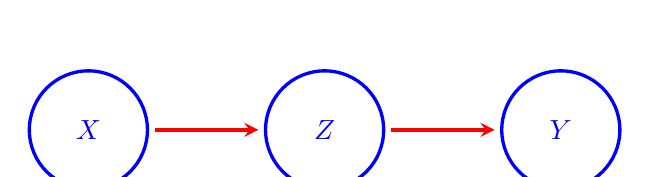
\begin{tikzpicture}
			\node[draw,circle,minimum size=1.5cm,minimum width=1.5cm,color=blue,very thick] (p1) at (0,0){$X$};
			\node[draw,circle,minimum size=1.5cm,minimum width=1.5cm,color=blue,very thick] (p2) at (3,0){$Z$};
			\node[draw,circle,minimum size=1.5cm,minimum width=1.5cm,color=blue,very thick] (p3) at (6,0){$Y$};
			\draw (p1) edge [->,>=stealth,shorten <=2pt, shorten >=2pt, very thick, color = red] (p2); 
			\draw (p2) edge [->,>=stealth,shorten <=2pt, shorten >=2pt, very thick, color = red] (p3); 
		\end{tikzpicture}
		\captionsetup{width=.7\linewidth}
		\caption{Example 2 of conditional independence.}
		\label{fig-conditional-indep-2}
	\end{figure}
	
	The corresponding joint pdf can be factorized as 
	\begin{align*}
		f_{X, Y, Z} \parens{x, y, z} = f_{X} \parens{x} f_{Z \vert X} \parens{z \,\vert\, x} f_{Y \vert Z} \parens{y \,\vert\, z}. 
	\end{align*}
	Marginalizing with respect to $Z$ yields 
	\begin{align*}
		f_{X, Y} \parens{x, y} = \int f_{X, Y, Z} \parens{x, y, z} \diff z = & \, f_{X} \parens{x} \int f_{Z \vert X} \parens{z \,\vert\, x} f_{Y \vert Z} \parens{y \,\vert\, z} \diff z \\ 
		= & \, f_{X} \parens{x} f_{Y \vert X} \parens{y \,\vert\, x}, 
	\end{align*}
	which, in general, cannot be factorized into $f_X \parens{x} f_Y \parens{y}$ and so $X$ and $Y$ are \emph{not} independent. 

	Now, conditioning on $Z$, we have 
	\begin{align*}
		f_{X, Y \vert Z} = \frac{f_{X, Y, Z} \parens{x, y, z}}{f_{Z} \parens{z}} = \frac{f_{X} \parens{x} f_{Z \vert X} \parens{z \,\vert\, x} f_{Y \vert Z} \parens{y \,\vert\, z}}{f_Z \parens{z}} = f_{X \vert Z} \parens{x \,\vert\, z} f_{Y \vert Z} \parens{y \,\vert\, z}, 
	\end{align*}
	and we obtain $X \indep Y \,\vert\, Z$. 
	
	\textit{Remark.} The node $Z$ is said to be \emph{head-to-tail} with respect to the path from node $X$ to node $Y$. Such a path connects nodes $X$ and $Y$ and renders them dependent. 
	
	\item \textbf{Example 3:} Consider the example shown in Figure \ref{fig-conditional-indep-3}. 
	
	\begin{figure}[h]
		\centering
		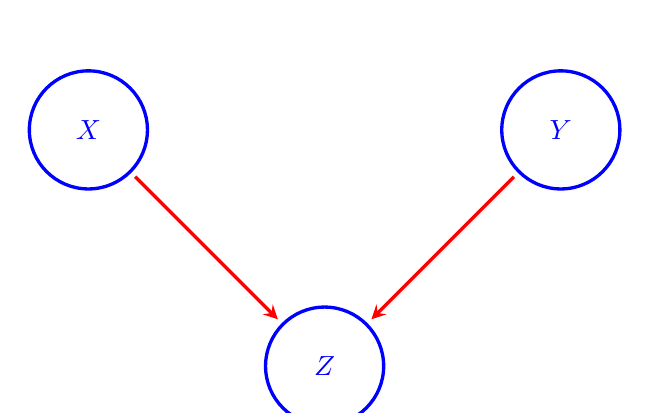
\begin{tikzpicture}
			\node[draw,circle,minimum size=1.5cm,minimum width=1.5cm,color=blue,very thick] (p1) at (0,0){$X$};
			\node[draw,circle,minimum size=1.5cm,minimum width=1.5cm,color=blue,very thick] (p2) at (6,0){$Y$};
			\node[draw,circle,minimum size=1.5cm,minimum width=1.5cm,color=blue,very thick] (p3) at (3,-3){$Z$};
			\draw (p1) edge [->,>=stealth,shorten <=2pt, shorten >=2pt, very thick, color = red] (p3); 
			\draw (p2) edge [->,>=stealth,shorten <=2pt, shorten >=2pt, very thick, color = red] (p3); 
		\end{tikzpicture}
		\captionsetup{width=.7\linewidth}
		\caption{Example 3 of conditional independence.}
		\label{fig-conditional-indep-3}
	\end{figure}
	
	The corresponding joint pdf can be factorized as 
	\begin{align*}
		f_{X, Y, Z} \parens{x, y, z} = f_{X} \parens{x} f_{Y} \parens{y} f_{Z \vert X, Y} \parens{z \,\vert\, x, y}. 
	\end{align*}
	Marginalizing with respect to $Z$ yields 
	\begin{align*}
		f_{X, Y} \parens{x, y} = \int f_{X, Y, Z} \parens{x, y, z} \diff z = & \, \int f_{X} \parens{x} f_{Y} \parens{y} f_{Z \vert X, Y} \parens{z \,\vert\, x, y} \diff z = f_{X} \parens{x} f_{Y} \parens{y}, 
	\end{align*}
	which states $X$ and $Y$ are independent. 
	
	Now, conditioning on $Z$, we have 
	\begin{align*}
		f_{X, Y \vert Z} = \frac{f_{X, Y, Z} \parens{x, y, z}}{f_{Z} \parens{z}} = \frac{f_{X} \parens{x} f_{Y} \parens{y} f_{Z \vert X, Y} \parens{z \,\vert\, x, y}}{f_Z \parens{z}}, 
	\end{align*}
	which, in general, cannot be factored into $f_{X \vert Z} \parens{x \,\vert\, z} f_{Y \vert Z} \parens{y \,\vert\, z}$. 
	
	\textit{Remark.} The node $Z$ is \emph{head-to-head} with respect to the path from $X$ to $Y$ because it connects to the heads of the two arrows. When node $Z$ is unobserved, it ``blocks'' the path, and the variables $X$ and $Y$ are independent. However, conditioning on $Z$ ``unblocks'' the path and renders $X$ and $Y$ dependent. 
	
	\item \textbf{Descendant:} We say that node $Y$ is a \emph{descendant} of node $X$ if there is a path from $X$ to $Y$ in which each step of the path follows the directions of the arrows. 
		
	\item \textbf{Summary:} 
	\begin{enumerate}
		\item A tail-to-tail node or a head-to-tail node leaves a path unblocked unless it is observed in which case it blocks the path; 
		\item A head-to-head node blocks a path if it is unobserved, but once the node, and/or at least one of its descendants, is observed, the path becomes unblocked. 
	\end{enumerate}
	
	\item \textbf{D-Separation:} Consider a directed acyclic graph in which $A$, $B$, and $C$ are arbitrary non-overlapping sets of nodes (whose union may be smaller than the complete set of nodes in the graph), and consider all possible paths from any node in $A$ to any node in $B$. Any such path is said to be \emph{blocked} if it includes a node such that either 
	\begin{enumerate}
		\item the arrows on the path meet either head-to-tail or tail-to-tail at the node, and the node is in the set $C$, or
		\item the arrows meet head-to-head at the node, and neither the node, nor any of its descendants, is in the set $C$. 
	\end{enumerate}
	If \emph{all} paths are blocked, then $A$ is said to be \emph{d-separated} from $B$ by $C$, and the joint distribution over all of the variables in the graph satisfies $A \indep B \,\vert\, C$. 

\end{enumerate}


\section*{IV. Undirected Graphs}


\subsection*{IV.1 Introduction}

\begin{enumerate}[label=\textbf{\arabic*.}]

	\item \textbf{Markov Random Field:} An \emph{undirected graph}, also knowns as a \emph{Markov random field} or a \emph{Markov network}, has 
	\begin{enumerate}
		\item a set of nodes each of which corresponds to a variable or group of variables, and 
		\item a set of edges each of which connects a pair of nodes. The edges are undirected, that is, they do \emph{not} carry arrows. 
	\end{enumerate}
	
	\item \textbf{Adjacent Vertices:} Two vertices $X$ and $Y$ are called \textit{adjacent} if there is an edge joining them, denoted by $X \sim Y$. 
	
	\item \textbf{Path:} A \textit{path} $X_1, X_2, \cdots, X_n$ is a set of vertices that are joined, that is, $X_{i-1} \sim X_i$ for $i = 2, \cdots, n$. 
	
	\item \textbf{Complete Graph:} A \textit{complete graph} is a graph with every pair of vertices joined by an edge. 
	
	\item \textbf{Subgraph:} A \textit{subgraph} $U \subset V$ is a subset of vertices together with their edges. 
	
	\item \textbf{Pairwise Markov Independence:} In a Markov random field $\calG$, the absence of an edge implies that the corresponding random variables are \textit{conditionally independent} given the variables at the other vertices; that is, 
	\begin{align}
		\text{no edge joining } X \text{ and } Y \iff X \indep Y \,\vert\, \text{rest}, 
	\end{align}
	where ``rest'' refers to all of the other vertices in the graph. These are known as the \emph{pairwise Markov independencies} of $\calG$. 
	
	\item \textbf{Separator:} If $A$, $B$ and $C$ are subgraphs, then $C$ is said to \textit{separate} $A$ and $B$ if every path between $A$ and $B$ intersects a node in $C$. The subgraph $C$ is said to be a \textit{separator}. 
	
	\item \textbf{Global Markov Properties:} Separators have the property that they break the graph into conditionally independent pieces. In a Markov random field $\calG$ with subgraphs $A$, $B$ and $C$, 
	\begin{align}
		\text{if $C$ separates $A$ and $B$, then $A \indep B \,\vert\, C$.}
	\end{align}
	This is known as the \textit{global Markov properties} of $\calG$. 
	
	\item \textbf{Equivalence of Pairwise and Global Markov Property:} The pairwise and global Markov properties of a graph are equivalent (for graphs with positive distributions). The set of graphs with associated probability distributions that satisfy the pairwise Markov independencies and global Markov properties are the same. 
	
	\textit{Remark.} The global Markov property allows us to decompose graphs into smaller more manageable pieces and leads to simplifications in computation and interpretation. 
	
	\item \textbf{Clique:} A \textit{clique} is a complete subgraph, i.e., a set of vertices in a graph such that there exists an edge between all pairs of vertices in the subset. In other words, the set of vertices in a clique is fully connected. 
	
	A clique is said to be \textit{maximal} if it is a clique and no other vertices can be added to it and still yield a clique. 
	
	\textit{Example.} Consider the graph in Figure \ref{fig-clique-example}. 
	\begin{figure}[h]
		\centering
		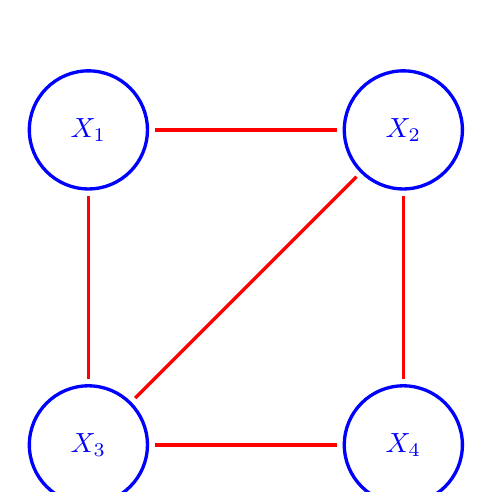
\begin{tikzpicture}
			\node[draw,circle,minimum size=1.5cm,minimum width=1.5cm,color=blue,very thick] (p1) at (0,0){$X_1$};
			\node[draw,circle,minimum size=1.5cm,minimum width=1.5cm,color=blue,very thick] (p2) at (4,0){$X_2$}; 
			\node[draw,circle,minimum size=1.5cm,minimum width=1.5cm,color=blue,very thick] (p3) at (0,-4){$X_3$}; 
			\node[draw,circle,minimum size=1.5cm,minimum width=1.5cm,color=blue,very thick] (p4) at (4,-4){$X_4$};
			\draw (p1) edge [-,>=stealth,shorten <=2pt, shorten >=2pt, very thick, color = red] (p3); 
			\draw (p1) edge [-,>=stealth,shorten <=2pt, shorten >=2pt, very thick, color = red] (p2); 
			\draw (p2) edge [-,>=stealth,shorten <=2pt, shorten >=2pt, very thick, color = red] (p3); 
			\draw (p2) edge [-,>=stealth,shorten <=2pt, shorten >=2pt, very thick, color = red] (p4); 
			\draw (p3) edge [-,>=stealth,shorten <=2pt, shorten >=2pt, very thick, color = red] (p4); 
		\end{tikzpicture}
		\captionsetup{width=.7\linewidth}
		\caption{Clique example.}
		\label{fig-clique-example}
	\end{figure}
	
	This graph has 
	\begin{enumerate}
		\item five cliques of two nodes given by $\sets{X_1, X_2}$, $\sets{X_2, X_3}$, $\sets{X_3, X_4}$, $\sets{X_4, X_2}$, and $\sets{X_1, X_3}$, and 
		\item two maximal cliques given by $\sets{X_1, X_2, X_3}$ and $\sets{X_2, X_3, X_4}$. 
	\end{enumerate}
	In particular, note that the set $\sets{X_1, X_2, X_3, X_4}$ is \emph{not} a clique. 
	
	\item \textbf{Implications on Density Factorization:} We can define the factors in the decomposition of the joint distribution of vertices in a graph to be functions of the variables in the \textit{maximal cliques}, without loss of generality, because other cliques must be subsets of maximal cliques. 
	
	\item \textbf{Probability Density Function over a Graph:} A probability density function $f$ over a Markov graph $\calG$ can be can represented as
	\begin{align}\label{clique.prod}
		f \parens{\bx} = \frac{1}{Z} \prod_{C \in \calC} \phi_C \parens{\bx_C}, 
	\end{align}
	where $\calC$ is the set of maximal cliques, and the positive functions $\psi_C \parens{\cdot}$ are called the \textit{clique potentials}. The quantity 
	\begin{align}\label{eq-partition-fun}
		Z := \int_{\calX} \prod_{C \in \calC} \psi_C \parens{\bx_C} \diff \bx 
	\end{align}
	is the normalizing constant, also known as the \textit{partition function}. 
	
	% Conversely, the representation \eqref{clique.prod} implies a graph with independence properties defined by the cliques in the product. 
	
	\textit{Remark 1.} We do \emph{not} require the choice of $\psi_C$'s to have a specific probabilistic interpretation as marginal or conditional distributions. 
		
	On the contrary, in directed graphs, each factor represents the conditional distribution of the corresponding variable, conditioned on the state of its parents. 
	
	\textit{Remark 2.} Since the choice of $\sets{\psi_C}$ is somewhat \textit{arbitrary}, their product will in general \emph{not} be correctly normalized. This is why we need $Z$ in \eqref{clique.prod}. 
		
	On the contrary, for directed graphs, the joint distribution was automatically normalized as a consequence of the normalization of each of the conditional distributions in the factorization. 
	
	\textit{Remark 3.} The presence of $Z$ in \eqref{clique.prod} is one of the major limitations of undirected graphs. The partition function $Z$ is needed for parameter estimation because it will be a function of any parameters that govern the potential functions. Its computation requires integration over a high-dimensional space. 
	
	For evaluation of \emph{local conditional distributions}, however, the partition function is \emph{not} needed because a conditional density function is the ratio of two marginals, and the partition function cancels when evaluating this ratio. 
		
	\item \textbf{Hammersley-Clifford Theorem:} Assume that each clique potential is strictly positive, i.e., $\psi_C \parens{\bx_C} > 0$ for all possible values of $\bx_C$. Let 
	\begin{enumerate}
		\item $S_1$ be the set of such distributions that are consistent with the set of conditional independence statements that can be read from the graph using graph separation, and 
		\item $S_2$ be the set of such distributions that can be expressed as a factorization of the form \eqref{clique.prod} with respect to the maximal cliques of the graph. 
	\end{enumerate}
	Then, the sets $S_1$ and $S_2$ are identical. 
	
	\textit{Remark.} Hammersley-Clifford theorem made the formal connection between conditional independence and factorization for undirected graphs. 
	
%	\item \textbf{Two General Comments:} 
%	\begin{enumerate}
%		\item A graphical model does not always uniquely specify the higher-order dependence structure of a joint probability distribution. 
%		
%		\begin{figure}[h]
%			\centering
%			\begin{tikzpicture}
%				\node[draw,circle,minimum size=1.5cm,minimum width=1.5cm,color=blue,very thick] (p1) at (0,2.5){$X$};
%				\node[draw,circle,minimum size=1.5cm,minimum width=1.5cm,color=blue,very thick] (p2) at (-2,0){$Y$}; 
%				\node[draw,circle,minimum size=1.5cm,minimum width=1.5cm,color=blue,very thick] (p3) at (2,0){$Z$}; 
%				\draw (p1) edge [-,>=stealth,shorten <=2pt, shorten >=2pt, very thick, color = red] (p3); 
%				\draw (p1) edge [-,>=stealth,shorten <=2pt, shorten >=2pt, very thick, color = red] (p2); 
%				\draw (p2) edge [-,>=stealth,shorten <=2pt, shorten >=2pt, very thick, color = red] (p3); 
%			\end{tikzpicture}
%			\captionsetup{width=.7\linewidth}
%			\caption{A complete graph does not uniquely specify the higher-order dependence structure in the joint distribution of the variables.}
%			\label{fig-nonuniqueness-example}
%		\end{figure}
%		
%		As an example, consider the complete three-node graph in Figure \ref{fig-nonuniqueness-example}. It could represent the dependence structure of either of the following distributions 
%		\begin{align*}
%			f_{X,Y,Z} \parens{x, y, z} = & \, \frac{1}{Z} \psi \parens{x, y} \psi \parens{x, z} \psi \parens{y, z}, \\ 
%			f_{X,Y,Z} \parens{x, y, z} = & \, \frac{1}{Z} \psi \parens{x, y, z}. 
%		\end{align*}
%		
%		\item Graphical models for discrete data are a special case of \textit{log-linear models} for \textit{multiway contingency tables}. 
%	\end{enumerate}

	\item \textbf{Energy Function:} Because we are restricted to potential functions which are \emph{strictly positive}, it is convenient to express them as exponentials, so that 
	\begin{align}
		\psi_C \parens{\bx_C} = \exp \parens[\big]{- E \parens{\bx_C}}, 
	\end{align}
	where $E$ is called an \emph{energy function}, and the exponential representation is called the \emph{Boltzmann distribution}. 
	
	\textit{Remark.} The joint distribution is defined as the product of potentials, and so the total energy is obtained by adding the energies of each of the maximal cliques. 

\end{enumerate}


\subsection*{IV.2 Relationships between Directed and Undirected Graphs}

\begin{enumerate}[label=\textbf{\arabic*.}]

	\item \textbf{Moralization:} In order to convert a directed graph into an undirected graph and convert any distribution specified by a factorization over a directed graph into one specified by a factorization over an undirected graph, we do the following: 
	\begin{enumerate}
		\item Add additional undirected links between \emph{all} pairs of parents for each node in the graph; 
		\item Drop the arrows on the original links; 
		\item Initialize all of the clique potentials of the moral graph to 1; 
		\item Take each conditional distribution factor in the original directed graph and multiply it into one of the clique potentials. 
	\end{enumerate}
	This process is called \textit{moralization}, and the resulting undirected graph is called a \textit{moral graph}. 
	
	\textit{Remark 1.} There will always exist at least one maximal clique that contains all of the variables in the factor as a result of the moralization step. 
	
	\textit{Remark 2.} In all cases, the partition function is given by $Z = 1$. 
	
	\textit{Remark 3.} When converting a directed graph into an undirected one, we could always \emph{trivially} convert any distribution over a directed graph into one over an undirected graph by simply using a fully connected undirected graph. This would, however, discard \emph{all} conditional independence properties and so would be useless. The process of moralization adds the \emph{fewest} extra edges and so retains the maximum number of independence properties. 
	
	\item \textbf{Example:} Consider the directed graph in the left panel in Figure \ref{fig-moral-example}. The joint distribution of the direct graph is 
	\begin{align*}
		f_{X_1, X_2, X_3, X_4} \parens{x_1, x_2, x_3, x_4} = f_{X_1} \parens{x_1} f_{X_2} \parens{x_2} f_{X_3} \parens{x_3} f_{X_4 \vert X_1, X_2, X_3} \parens{x_4 \,\vert\, x_1, x_2, x_3}. 
	\end{align*}
	Note that the last factor $f_{X_4 \vert X_1, X_2, X_3} \parens{x_4 \,\vert\, x_1, x_2, x_3}$ involves all four variables, and, hence, they all must belong to the single clique if this conditional distribution is absorbed into a clique potential. Therefore, we add extra edges between all pairs of parents of the vertex $X_4$. The resulting moral graph is shown in the right panel of Figure \ref{fig-moral-example} and the clique potential is 
	\begin{align*}
		\psi_C \parens{x_1, x_2, x_3, x_4} = f_{X_1, X_2, X_3, X_4} \parens{x_1, x_2, x_3, x_4}. 
	\end{align*}
	
	\begin{figure}[t]
		\centering
		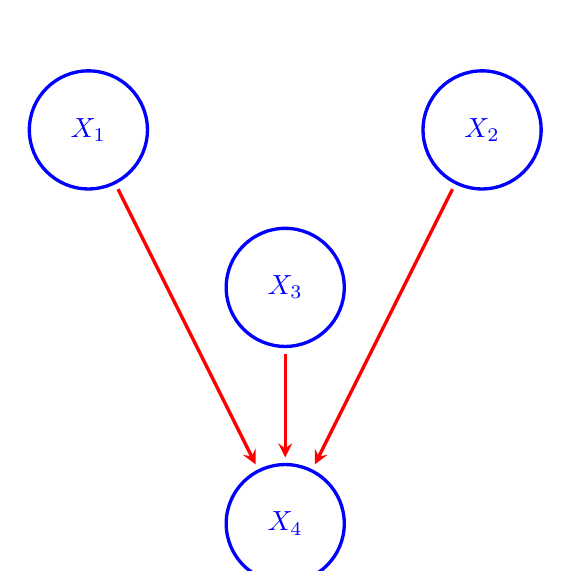
\begin{tikzpicture}
			\node[draw,circle,minimum size=1.5cm,minimum width=1.5cm,color=blue,very thick] (p1) at (0,0){$X_1$};
			\node[draw,circle,minimum size=1.5cm,minimum width=1.5cm,color=blue,very thick] (p2) at (5,0){$X_2$}; 
			\node[draw,circle,minimum size=1.5cm,minimum width=1.5cm,color=blue,very thick] (p3) at (2.5,-2){$X_3$}; 
			\node[draw,circle,minimum size=1.5cm,minimum width=1.5cm,color=blue,very thick] (p4) at (2.5,-5){$X_4$};
			\draw (p1) edge [->,>=stealth,shorten <=2pt, shorten >=2pt, very thick, color = red] (p4); 
			\draw (p2) edge [->,>=stealth,shorten <=2pt, shorten >=2pt, very thick, color = red] (p4); 
			\draw (p3) edge [->,>=stealth,shorten <=2pt, shorten >=2pt, very thick, color = red] (p4); 
		\end{tikzpicture}
		\qquad 
		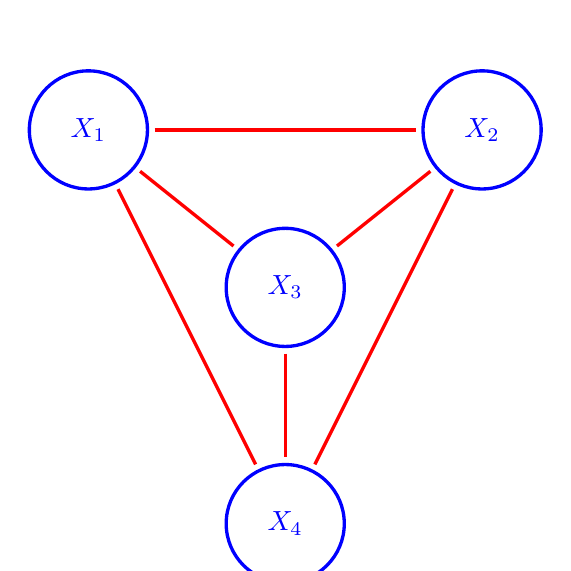
\begin{tikzpicture}
			\node[draw,circle,minimum size=1.5cm,minimum width=1.5cm,color=blue,very thick] (p1) at (0,0){$X_1$};
			\node[draw,circle,minimum size=1.5cm,minimum width=1.5cm,color=blue,very thick] (p2) at (5,0){$X_2$}; 
			\node[draw,circle,minimum size=1.5cm,minimum width=1.5cm,color=blue,very thick] (p3) at (2.5,-2){$X_3$}; 
			\node[draw,circle,minimum size=1.5cm,minimum width=1.5cm,color=blue,very thick] (p4) at (2.5,-5){$X_4$};
			\draw (p1) edge [-,>=stealth,shorten <=2pt, shorten >=2pt, very thick, color = red] (p3); 
			\draw (p1) edge [-,>=stealth,shorten <=2pt, shorten >=2pt, very thick, color = red] (p2); 
			\draw (p2) edge [-,>=stealth,shorten <=2pt, shorten >=2pt, very thick, color = red] (p3); 
			\draw (p2) edge [-,>=stealth,shorten <=2pt, shorten >=2pt, very thick, color = red] (p4); 
			\draw (p3) edge [-,>=stealth,shorten <=2pt, shorten >=2pt, very thick, color = red] (p4); 
			\draw (p1) edge [-,>=stealth,shorten <=2pt, shorten >=2pt, very thick, color = red] (p4); 
		\end{tikzpicture}
		\captionsetup{width=.7\linewidth}
		\caption{Moralization example.}
		\label{fig-moral-example}
	\end{figure}
	
	\textit{Remark.} In this particular example, the moral graph is fully connected and so exhibits \emph{no} conditional independence properties, in contrast to the original directed graph. 

\end{enumerate}


\section*{V. Undirected Graphical Models for Continuous Random Variables}

\subsection*{V.1 Introduction}

\begin{enumerate}[label=\textbf{\arabic*.}]

	\item \textbf{Setup:} In this section, we consider the undirected graphs where all the variables are continuous. 
	
	\item \textbf{Assumption:} Assume that the observations have a multivariate Gaussian distribution with mean $\bmu$ and covariance matrix $\bSigma$. 
	
	\textit{Remarks.}
	\begin{enumerate}
		\item Since the Gaussian distribution represents at most \textit{second-order} relationships, it automatically encodes a \textit{pairwise Markov graph}. 
		\item The Gaussian distribution has the property that all conditional distributions are also Gaussian. 
	\end{enumerate}
	
	\item \textbf{Inverse Covariance Matrix of a Gaussian Distribution and Conditional Independence:} 
	%The inverse covariance matrix, $\bSigma^{-1}$, contains information about the \textit{partial covariances} between the variables. 
	Suppose 
	\begin{align*}
		X = \parens{X_1, X_2, \cdots, X_p}^\top \sim \Normal_p \parens{\bmu_p, \bSigma}, 
	\end{align*}
	where $\bSigma \in \Real^{p \times p}$ is positive definite. If $\parens{i, j}$-th entry of $\bTheta := \bSigma^{-1}$ is zero, then $X_i$ and $X_j$ are conditionally independent, given all other variables. 
	
	\textit{Remark.} This result can be proved by working with the inverse of a block matrix and the conditional distribution of a Gaussian random vector. 
	
	\item \textbf{Conditional Gaussian Distribution:} Suppose we partition a $p$-dimensional random vector $X$ as $X = \parens{Z^\top, Y^\top}^\top$, where $Z = \parens{X_1, X_2, \cdots, X_{p-1}}^\top \in \Real^{p-1}$ consists of the first $\parens{p-1}$ components of $X$ and $Y = X_p$ is the last. Then, the conditional distribution of $Y$ given $Z = \bz$ is 
	\begin{align}\label{cond.dis}
		Y \,\vert\, Z = \bz \sim \Normal \, \parens[\big]{\mu_Y + \parens{\bz - \bmu_Z}^\top \bSigma_{ZZ}^{-1} \bSigma_{ZY}, \sigma_{YY} - \bSigma_{YZ} \bSigma_{ZZ}^{-1} \bSigma_{ZY}}, 
	\end{align}
	where the covariance matrix is partitioned as 
	\begin{align}
		\bSigma = \begin{pmatrix}
			\bSigma_{ZZ} & \bSigma_{ZY} \\ 
			\bSigma_{YZ} & \sigma_{YY}
		\end{pmatrix}. 
	\end{align}
	Notice that the conditional mean in \eqref{cond.dis} has exactly the same form as the population multiple linear regression of $Y$ on $Z$, with the regression coefficient $\bbeta = \bSigma_{ZZ}^{-1} \bSigma_{ZY}$. 
	
	If we partition the inverse covariance matrix $\bTheta = \bSigma^{-1}$ in a similar fashion, we have 
	\begin{align}
		\bTheta_{ZY} = - \theta_{YY} \bSigma_{ZZ}^{-1} \bSigma_{ZY}, 
	\end{align}
	where $\theta_{YY}^{-1} = \sigma_{YY} - \bSigma_{YZ} \bSigma_{ZZ}^{-1} \bSigma_{ZY} > 0$. It follows that 
	\begin{align}
		\bbeta = \bSigma_{ZZ}^{-1} \bSigma_{ZY} = - \frac{\bTheta_{ZY}}{\theta_{YY}}. 
	\end{align}
	
	\item \textbf{$\bTheta$ as the Natural Parameter:} The inverse covariance matrix $\bTheta$ captures \emph{all} the second-order structural and quantitative information to describe the conditional distribution of each node given the rest. 
	
	The distribution arising from a Gaussian graphical model is a \textit{Wishart distribution}, and is a member of the exponential family, with canonical or ``natural'' parameter being $\bTheta = \bSigma^{-1}$. 

\end{enumerate}


\subsection*{V.2 Estimation of the Parameters when the Graph Structure is Known}

\begin{enumerate}[label=\textbf{\arabic*.}]

	\item \textbf{Complete Graph Case:} 
	\begin{enumerate}
		\item \textit{Assumptions:} We assume the graph is complete, i.e., the graph is fully connected. 
		
		\item \textit{Data:} Suppose we have $n$ multivariate normal realizations $\bx_i \in \Real^p$, for $i = 1, 2, \cdots, n$, with population mean and covariance $\bSigma$. 
		
		\item \textit{Sample Covariance Matrix:} Let $\bS \in \Real^{p \times p}$ be the empirical covariance matrix, where 
		\begin{align}
			\bS = \frac{1}{n} \sum_{i=1}^n \parens{\bx_i - \bar{\bx}} \parens{\bx_i - \bar{\bx}}^\top, 
		\end{align} 
		and $\bar{\bx} = \frac{1}{n} \sum_{i=1}^n \bx_i$ is the sample mean vector. 
		
		\item \textit{Log-likelihood Function and MLE of $\bTheta$:} The log-likelihood function of $\bTheta$ is 
		\begin{align}
			\ell \parens{\bTheta} = \log \det \parens{\bTheta} - \trace \parens{\bS \bTheta}. 
		\end{align}
		The quantity $-\ell$ is a convex function of $\bTheta$, and it is easy to show the maximum likelihood estimate of $\bTheta$ is $\bS^{-1}$. It follows that the maximum likelihood estimate of $\bSigma$ is $\bS$. 
		
	\end{enumerate}
	
	\item \textbf{Incomplete Graph with Known Structure:} 
	\begin{enumerate}
		\item \textit{Setup:} In the incomplete graph case, some of the edges are missing, implying that the corresponding entries of $\bTheta = \bSigma^{-1}$ are 0 in the Gaussian distribution case. 
		
		\item \textit{General Approach:} We maximize the likelihood function under the constraints that some pre-defined subset of the parameters are zero, which is an equality-constrained convex optimization problem. 
		
		\textit{Remark.} The central idea of the approach described above is to decompose the graph into its \textit{maximal cliques}. 
		
		\item \textit{Optimization Problem:} We maximize the following constrained log-likelihood function 
		\begin{align}\label{constrained.loglik}
			\ell_C \parens{\bTheta} = \log \det \parens{\bTheta} - \trace \parens{\bS \bTheta} - \sum_{\parens{j, k} \notin E} \gamma_{j,k}\theta_{j,k}, 
		\end{align}
		where the last term $\sum_{\parens{j, k} \notin E} \gamma_{j, k}\theta_{j,k}$ restricts the $\parens{j, k}$-th entry of $\bTheta$ to be zero and reflects the known graph structure there is no edge between the corresponding variables. 
		
		The first-order optimality condition of maximizing $\ell_C$ requires 
		\begin{align}\label{opt.condition}
			\bTheta^{-1} - \bS - \bGamma = \boldzero_{p \times p}, 
		\end{align}
		where $\bGamma$ is a matrix of Lagrange parameters with nonzero values for all pairs with edges absent. In deriving \eqref{opt.condition}, we use the fact that the derivative of $\log \det \parens{\bTheta}$ is $\bTheta^{-1}$. 
		
		\item \textit{Characterizing the Solution:} Let $\bW = \bTheta^{-1}$. Without the loss of generality, we partition the matrix $\bW \in \Real^{p \times p}$ as 
		\begin{align*}
			\bW = \begin{pmatrix}
				\bW_{11} & w_{12} \\ 
				w_{21} & w_{22}
			\end{pmatrix}
		\end{align*}
		and look at the last column and the last row of $\bW$. We have 
		\begin{align}\label{eq-17.15}
			\bW \bTheta = \begin{pmatrix}
				\bW_{11} & \bW_{12} \\ 
				\bW_{21} & w_{22}
			\end{pmatrix} \begin{pmatrix}
				\bTheta_{11} & \bTheta_{12} \\ 
				\bTheta_{21} & \theta_{22}
			\end{pmatrix} = \begin{pmatrix}
				\bI_{\parens{p-1} \times \parens{p-1}} & \boldzero_{p-1} \\ \boldzero_{p-1}^\top & 1
			\end{pmatrix}. 
		\end{align}
		Therefore, we must have 
		\begin{align*}
			\bW_{11} \bTheta_{12} + \bW_{12} \theta_{22} = 0, 
		\end{align*}
		from which we obtain 
		\begin{align*}
			\bW_{12} = - \bW_{11} \frac{\bTheta_{12}}{\theta_{22}} = \bW_{11} \bbeta, 
		\end{align*}
		where $\bbeta = - \frac{\bTheta_{12}}{\theta_{22}} \in \Real^{p-1}$. From \eqref{opt.condition}, using a similar partition of the matrices $\bS$ and $\bGamma$, it follows that 
		\begin{align}\label{eq-17.18}
			\boldzero_{p-1} = \bW_{12} - \bS_{12} - \bGamma_{12} = \bW_{11} \bbeta - \bS_{12} - \bGamma_{12}. 
		\end{align}
		To solve this equation, suppose that there are $p - q - 1$ non-zero elements in $\bGamma_{12}$, i.e., $p - q - 1$ edges are constrained to be zero. Then, these $p - q - 1$ rows carry no information and can be removed. Consequently, we can reduce $\bbeta$ to $\widetilde{\bbeta}$ by removing the corresponding $p - q - 1$ zero elements and obtain the following reduced $q \times q$ system of equations 
		\begin{align}\label{17.19}
			\widetilde{\bW}_{11} \widetilde{\bbeta} - \widetilde{\bS}_{12} = \boldzero_{q}, 
		\end{align}
		from which we have $\widetilde{\bbeta} = \widetilde{\bW}_{11}^{-1} \widetilde{\bS}_{12}$. To obtain $\bbeta$ that satisfies \eqref{eq-17.18}, simply insert zeros at appropriate positions. 
		
		It is easy to obtain from \eqref{eq-17.15} that 
		\begin{align*}
			\bW_{12} \bTheta_{12} + w_{22} \theta_{22} = 1, 
		\end{align*}
		from which we can solve 
		\begin{align*}
			\frac{1}{\theta_{22}} = w_{22} - \bW_{12}^\top \bbeta. 
		\end{align*}
		Finally, we have $w_{22} = s_{22}$, since the diagonal of $\bGamma$ is zero. 
		
		\item \textit{Algorithm:} The arguments above lead to a simple iterative procedure for estimating both $\bW$ and its inverse $\bTheta$, subject to the constraints of the missing edges. The complete iterative algorithm is shown in Algorithm \ref{algo-modified-regres}. 
		
		\begin{minipage}{\linewidth}
			\begin{algorithm}[H]
				\caption{A Modified Regression Algorithm for Estimation of an Undirected Gaussian Graphical Model with Known Structure}\label{algo-modified-regres}
				\begin{algorithmic}[1]
					\STATE Initialize $\bW = \bS$; 
					
					\REPEAT{}
					\FOR{$j = 1, 2, \cdots, p$}
					\STATE Partition the matrix $\bW$ into one part containing all but the $j$-th row and column and the other part containing the $j$-th row and column; 
					\STATE Solve 
					\begin{align*}
						\widetilde{\bW}_{11} \widetilde{\bbeta} - \widetilde{\bS}_{12} = \boldzero
					\end{align*}
					for the unconstrained edge parameters $\widetilde{\bbeta}$, using the reduced system of equations as in \eqref{17.19}; 
					\STATE Obtain $\bbeta$ that satisfies \eqref{eq-17.18} by padding $\widetilde{\bbeta}$ with zeros in the appropriate positions; 
					\STATE Update $\bW_{12} = \bW_{11} \bbeta$; 
					\ENDFOR
					\UNTIL{convergence}
					
					\STATE In the final cycle for each $j$, solve for 
					\begin{align*}
						\bTheta_{12} = - \bbeta \theta_{22}, \qquad w_{22} = s_{22}, \qquad  \text{ and } \qquad \theta_{22}^{-1} = w_{22} - \bW_{12}^\top \bbeta. 
					\end{align*}
				
				\end{algorithmic}
			\end{algorithm}
		\end{minipage}
	\end{enumerate}

\end{enumerate}


\subsection*{V.3 Estimation of Graph Structure}

\begin{enumerate}[label=\textbf{\arabic*.}]

	\item \textbf{Motivation:} In most cases of applications, we do \emph{not} know the exact graph structure or the missing edges, and would like to try to discover from the data. 
	
	\item \textbf{General Idea:} The general idea is that, rather than estimating the full covariance $\bSigma$ or its inverse $\bTheta = \bSigma^{-1}$, only estimate which components of $\theta_{i,j}$ are non-zero, by fitting a lasso regression using each variance as the response and the others as predictors. 
	
	\item \textbf{Lasso-Type Optimization Problem:} The idea above leads to the problem of maximizing the penalized log-likelihood function 
	\begin{align}\label{17.21}
		\ell_{\mathrm{lasso}} \parens{\bTheta} := \log \det \parens{\bTheta} - \trace\parens{\bS \bTheta} - \lambda \cdot \norm{\bTheta}_1, 
	\end{align}
	where $\norm{\bTheta}_1$ is the $L^1$-norm, the sum of the absolute values of the elements in $\bTheta = \bSigma^{-1}$. Notice that the negative of \eqref{17.21} is a convex function of $\bTheta$. 
	
	The gradient of $\ell_{\mathrm{lasso}}$ is 
	\begin{align*}
		\bTheta^{-1} - \bS - \lambda \cdot \sign \parens{\bTheta} = \boldzero_{p \times p}, 
	\end{align*}
	where the sign function is applied entry-wise with 
	\begin{align*}
		\sign \parens{\theta} = \begin{cases}
			-1, & \, \text{ if } \theta < 0, \\ 
			\bracks{-1, 1}, & \, \text{ if } \theta = 0, \\ 
			+1, & \, \text{ if } \theta > 0. \\ 
		\end{cases}
	\end{align*}
	By letting $\bW = \bTheta^{-1}$ and partitioning $\bW$ in a similar fashion to the previous section, we have 
	\begin{align}
		\bW_{11} \bbeta - \bS_{12} + \lambda \cdot \sign \parens{\bbeta} = \boldzero_{p-1}, 
	\end{align}
	where we flip the sign in the last term since $\bbeta = - \frac{\bTheta_{12}}{\theta_{22}}$ and $\bbeta$ and $\bTheta_{12}$ have opposite signs. 
	
	To proceed, we use the coordinate descent method at each stage. Let $\bV = \bW_{11}$, the update has the form 
	\begin{align}
		\beta_j \quad \longleftarrow \quad S_{\lambda} \parens[\Bigg]{s_{12,j} - \sum_{k \neq j} v_{k,j}\beta_k} / V_{jj}, 
	\end{align}
	for $j = 1, 2, \cdots, p-1$, where $s_{12,j}$ is the $j$-th element of $\bS_{12}$, $v_{k,j}$ is the $\parens{k, j}$-th entry of $\bV$, and $S_{\lambda}$ is the soft-thresholding operator 
	\begin{align*}
		S_{\lambda} \parens{x} = \sign \parens{x} \cdot \parens{\abs{x} - \lambda}_+. 
	\end{align*}
	The diagonal elements $w_{jj}$ of the matrix $\bW$ are simply $s_{jj} + \lambda$ and are fixed. 
	
	\item \textbf{Graphical Lasso Algorithm:} The entire algorithm of solving $\bTheta$ is called \textit{graphical lasso}, summarized in Algorithm \ref{glasso}. 
	
	\begin{minipage}{\linewidth}
		\begin{algorithm}[H]
			\caption{Graphical Lasso}\label{glasso}
			\begin{algorithmic}[1]
				\STATE Initialize $\bW = \bS + \lambda \cdot \bI_p$. The diagonal of $\bW$ remains unchanged in the following steps; 
				\REPEAT
				\FOR{$j = 1, 2, \cdots, p$}
				\STATE Partition the matrix $\bW$ into one part containing all but the $j$th row and column and the other part containing the $j$th row and column; 
				\STATE Solve the estimated equations 
				\begin{align*}
					\bW_{11} \bbeta - \bS_{12} + \lambda \cdot \sign \parens{\bbeta} = \boldzero_{p-1}; 
				\end{align*}
				\STATE Update $\bW_{12} = \bW_{11} \bbeta$; 
				\ENDFOR
				\UNTIL{convergence}
				\STATE In the final cycle for each $j$, solve for 
				\begin{align*}
					\theta_{22}^{-1} = s_{22} - \bW_{12}^\top \beta \qquad \text{ and } \qquad \bTheta_{12} = - \bbeta \theta_{22}.  
				\end{align*}
			\end{algorithmic}
		\end{algorithm}
	\end{minipage}

\end{enumerate}


\section*{VI. Undirected Graphical Models for Discrete Variables}

\begin{enumerate}[label=\textbf{\arabic*.}]

	\item \textbf{General Introductions:} 
	\begin{enumerate}
		\item The pairwise Markov networks with binary variables are called the \textit{Ising models} in the statistical mechanics literature, and the \textit{Boltzmann machines} in the machine learning literature. 
		\item The values at each node can be observed (``visible'') or unobserved (``hidden''). Nodes are organized in layers, similar to neural networks. 
	\end{enumerate}
	
	\item \textbf{Ising Model 1 --- Introduction:} Consider all $p$ nodes in a graph $\calG = \parens{V, E}$ are visible with edges pairs $\parens{j, k}$ enumerated in $E$, and let the binary-valued variable at node $j$ be $X_j$. The \textit{Ising model} for their joint probabilities is given by 
	\begin{align}
		\Pr_{\bTheta} \parens{X = \bx} = \exp \bracks[\Bigg]{\sum_{ \parens{j, k} \in E} \theta_{j,k} x_j x_k - \Phi \parens{\bTheta}}, 
	\end{align}
	for $\bx = \parens{x_1, x_2, \cdots, x_p}^\top \in \calX := \braces{0, 1}^p$. Here, $\Phi$ is the log-partition function defined as 
	\begin{align}
		\Phi \parens{\bTheta} = \log \bracks[\Bigg]{\sum_{\bx \in \calX} \exp \parens[\bigg]{\sum_{\parens{j, k} \in E} \theta_{j, k} x_j x_k}}, 
	\end{align}
	ensuring the probability mass function add to one over $\calX$. 
	
	\textit{Remark 1.} We require a \textit{constant node} $X_0 = 1$ to be included with ``edges'' to all the other variables. 
	
	\textit{Remark 2.} In statistical literature, the Ising model is equivalent to a first-order-interaction Poisson log-linear model for multiway tables of counts. 
	
	\item \textbf{Ising Model 2 --- Conditional Probability Mass Function:} For each node conditional on others, the corresponding conditional probability mass function takes on the form 
	\begin{align}
		\Pr_{\bTheta} \parens{X_j = 1 \,\vert\, X_{-j} = \bx_{-j}} = \frac{1}{1 + \exp \parens{-\theta_{j,0} - \sum_{\parens{j, k} \in E} \theta_{j, k} x_k}}, 
	\end{align}
	where $X_{-j}$ denotes all of the nodes except $X_j$ and $\bx_{-j}$ denotes the observed value of $X_{-j}$. Here, the parameter $\theta_{j,k}$ measures the dependence of $X_j$ on $X_k$, conditional on other nodes. 
	
	\item \textbf{Ising Model 3 --- Estimation of Parameters When Graph Structure is Known:} Suppose we have the observations $\bx_i = \parens{x_{i,1}, x_{i,2}, \cdots, x_{i,p}}^\top \in \calX$ for $i = 1, 2, \cdots, n$. The average log-likelihood is 
	\begin{align}
		\ell \parens{\bTheta} = \frac{1}{n} \sum_{i=1}^n \log \Pr_{\bTheta} \parens{X = \bx_i} = \frac{1}{n} \sum_{i=1}^n \bracks[\Bigg]{\sum_{\parens{j, k} \in E} \theta_{j,k} x_{i,j} x_{i, k} - \Phi \parens{\bTheta}}. 
	\end{align}
	The gradient of the log-likelihood is 
	\begin{align*}
		\frac{\partial \ell \parens{\bTheta}}{\partial \theta_{j,k}} = \frac{1}{n} \sum_{i=1}^n x_{i,j} x_{i,k} - \frac{\partial \Phi \parens{\bTheta}}{\partial \theta_{j,k}}, 
	\end{align*}
	and 
	\begin{align*}
		\frac{\partial \Phi \parens{\bTheta}}{\partial \theta_{j,k}} = \sum_{\bx \in \calX} x_j x_k \Pr_{\bTheta} \parens{X = \bx} = \E_{\bTheta}\bracks{X_j X_k}. 
	\end{align*}
	Setting the gradient to 0, we obtain 
	\begin{align}\label{17.34}
		\widehat{\E} \bracks{X_j X_k} - \E_{\widehat{\bTheta}} \bracks{X_j X_k} = 0, 
	\end{align}
	where $\widehat{\bTheta}$ is the maximum likelihood estimate of $\bTheta$ and 
	\begin{align*}
		\widehat{\E} \bracks{X_j X_k} = \frac{1}{n} \sum_{i=1}^n x_{i,j} x_{i,k},  
	\end{align*}
	is the expectation taken with respect to the empirical distribution of the data. The central idea of \eqref{17.34} is that the maximum likelihood estimates match the estimated inner products between the nodes to their observed inner products. 
	
	\textit{Computation of $\widehat{\bTheta}$:} To obtain $\widehat{\bTheta}$, we can use the gradient descent algorithm or Newton's method. However, the computation of $\E_{\bTheta} \bracks{X_j X_k}$ involves enumeration of $\Pr_{\bTheta} \parens{X}$ over $2^{p-2}$ of the $\abs{\calX} = 2^p$ possible values of $X$, which is infeasible for large $p$. % For small $p$, one can use Poisson log-linear regression, gradient descent, or iterative proportional fitting. 
	
	\item \textbf{Hidden Nodes:} Suppose that a subset of variables $X_{\mathrm{mis}}$ are unobserved or ``hidden'', and the remainder $X_{\mathrm{obs}}$ are observed or ``visible''. The log-likelihood of the observed data is 
	\begin{align*}
		\ell \parens{\bTheta} = & \, \sum_{i=1}^n \log \Pr_{\bTheta} \parens{X_{\mathrm{obs}} = x_{i, \mathrm{obs}}} \\ 
		= & \, \sum_{i=1}^n \log \bracks[\Bigg]{\sum_{\bx_{\mathrm{mis}} \in \calX_{\mathrm{mis}}} \exp \parens[\bigg]{\sum_{\parens{j, k} \in E} \parens{\theta_{j, k} x_{i, j} x_{i, k} - \Phi \parens{\bTheta}}}}, 
	\end{align*}
	where the sum over $\calX_{\mathrm{mis}}$ means that we are summing over all possible $\braces{0, 1}$ values for the hidden units. 
	
	The gradient of $\ell$ with respect to $\theta_{j,k}$ is 
	\begin{align}
		\frac{\partial \ell \parens{\bTheta}}{\partial \theta_{j,k}} = \widehat{\E}_{\mathrm{obs}}\bracks[\big]{\E_{\bTheta} \bracks{X_j X_k \,\vert\, X_{\mathrm{obs}}}} - \E_{\bTheta} \bracks{X_j X_k}, 
	\end{align}
	where 
	\begin{enumerate}
		\item the first term is an empirical average of $X_jX_k$ if both are visible; if one or both are hidden, they are first imputed given the visible data, and then averaged over the hidden variables; 
		\item the second term is the unconditional expectation of $X_jX_k$.  
	\end{enumerate}
	The inner expectation in the first term can be evaluated in the following way: for observation $i$, 
	\begin{enumerate}
		\item if both $j$-th and $k$-th components are observed, then 
		\begin{align*}
			\E_{\bTheta} \bracks{X_j X_k \,\vert\, X_{\mathrm{obs}} = \bx_{i, \mathrm{obs}}} = x_{i,j} x_{i,k}; 
		\end{align*}
		\item if the $j$-th component is observed but the $k$-th component is hidden, then 
		\begin{align*}
			\E_{\bTheta} \bracks{X_j X_k \,\vert\, X_{\mathrm{obs}} = \bx_{i, \mathrm{obs}}} = x_{i,j} \Pr_{\bTheta} \parens{X_k = 1 \,\vert\, X_{\mathrm{obs}} = \bx_{i, \mathrm{obs}}}; 
		\end{align*}
		\item if both $j$-th and $k$-th components are hidden, then 
		\begin{align*}
			\E_{\bTheta} \bracks{X_j X_k \,\vert\, X_{\mathrm{obs}} = \bx_{i, \mathrm{obs}}} = \Pr_{\bTheta}\parens{X_j = 1, X_k = 1 \,\vert\, X_{\mathrm{obs}} = \bx_{i, \mathrm{obs}}}. 
		\end{align*}
	\end{enumerate}
	
\end{enumerate}

\printbibliography

\end{document}
